\documentclass[aspectratio=1610,8pt]{beamer}

% Standard packages

\usepackage[english]{babel}
\usepackage{siunitx}
\usepackage{textcomp}
%\usepackage[latin1]{inputenc}
%\usepackage{times}
%\usepackage[T1]{fontenc}


% Setup TikZ

\usepackage{tikz}
\usetikzlibrary{arrows}
%\tikzstyle{block}=[draw opacity=0.7,line width=1.4cm]


% Author, Title, etc.

\title{Queue using Linked List}

\author[Shiv Shankar Dayal]{Shiv Shankar Dayal}

% The main document

\begin{document}
\begin{frame}[fragile]
  \titlepage
\end{frame}
\begin{frame}[fragile]{Enqueue when Head and Tail are NULL}
  Enqueue operation when both head and tail are \texttt{NULL}. First
  we malloc a node temp which is having grabage data and pointer
  pointing to a not so useful location. Let us say we want to
  enqueue data \texttt{10}.
  \begin{center}
    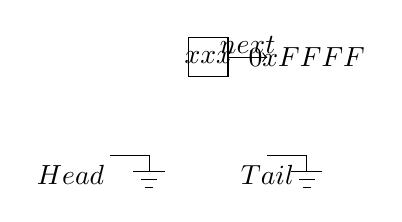
\begin{tikzpicture}
      \draw (0,0) rectangle(.5, .5);
      \draw (.25, .25) node{$xxx$};
      \draw (-1, -1) -- (-.5, -1) -- (-.5, -1.2);
      \draw (1, -1) -- (1.5, -1) -- (1.5, -1.2);
      \draw[->] (.5, .25) -- (1, .25);
      \draw (.75, .4) node{$next$};
      \draw (1.5, .25) node{$0xFFFF$};
      \draw (-1.5, -1) node[anchor=north]{$Head$};
      \draw (1, -1) node[anchor=north]{$Tail$};
      \draw (-.7, -1.2) -- (-.3, -1.2);
      \draw (-.6, -1.3) -- (-.4, -1.3);
      \draw (-.55, -1.4) -- (-.45, -1.4);
      \draw (1.7, -1.2) -- (1.3, -1.2);
      \draw (1.6, -1.3) -- (1.4, -1.3);
      \draw (1.55, -1.4) -- (1.45, -1.4);
    \end{tikzpicture}
  \end{center}
\end{frame}
\begin{frame}[fragile]{Enqueue when Head and Tail are NULL}
  We set the data in allocated node and set \texttt{next} to \texttt{NULL}.
  Then make head and tail both point to it.
  \begin{center}
    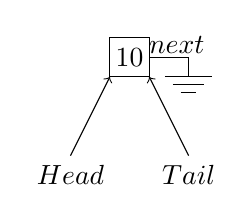
\begin{tikzpicture}
      \draw (0, 0) rectangle(.5, .5);
      \draw (.25, .25) node{$10$};
      \draw (.5, .25) -- (1, .25) -- (1, 0);
      \draw (.85, .4) node{$next$};
      \draw (.7, 0) -- (1.3, 0);
      \draw (.8, -.1) -- (1.2, -.1);
      \draw (.9, -.2) -- (1.1, -.2);
      \draw (-.5, -1) node[anchor=north]{$Head$};
      \draw (1, -1) node[anchor=north]{$Tail$};
      \draw[->] (-.5, -1) -- (0, 0);
      \draw[->] (1, -1) -- (.5, .0);
    \end{tikzpicture}
  \end{center}
\end{frame}
\begin{frame}[fragile]{Enqueue when Head and Tail are not NULL}
  Let us say we want to enqueue 20. We allocate a new node set the data in
  allocated node and set \texttt{next} to \texttt{NULL}.
  \begin{center}
    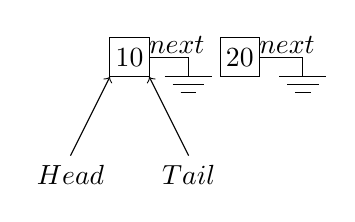
\begin{tikzpicture}
      \draw (0, 0) rectangle(.5, .5);
      \draw (.25, .25) node{$10$};
      \draw (.5, .25) -- (1, .25) -- (1, 0);
      \draw (.85, .4) node{$next$};
      \draw (.7, 0) -- (1.3, 0);
      \draw (.8, -.1) -- (1.2, -.1);
      \draw (.9, -.2) -- (1.1, -.2);
      \draw (-.5, -1) node[anchor=north]{$Head$};
      \draw (1, -1) node[anchor=north]{$Tail$};
      \draw[->] (-.5, -1) -- (0, 0);
      \draw[->] (1, -1) -- (.5, 0);
      
      \draw (1.4, 0) -- (1.9, 0) -- (1.9, .5) -- (1.4, .5) --cycle;
      \draw (1.65, .25) node{$20$};
      \draw (2.25, .4) node{$next$};
      \draw (.7, 0) -- (1.3, 0);
      \draw (.8, -.1) -- (1.2, -.1);
      \draw (.9, -.2) -- (1.1, -.2);
      \draw (1.9, .25) -- (2.45, .25) -- (2.45, 0);
      \draw (2.15, 0) -- (2.75, -0);
      \draw (2.25, -.1) -- (2.65, -.1);
      \draw (2.35, -.2) -- (2.55, -.2);
    \end{tikzpicture}
  \end{center}
\end{frame}
\begin{frame}[fragile]{Enqueue when Head and Tail are not NULL}
  Now we point \texttt{next} of \texttt{tail} to this new allocated item
  and set \texttt{tail} to point to it.
  \begin{center}
    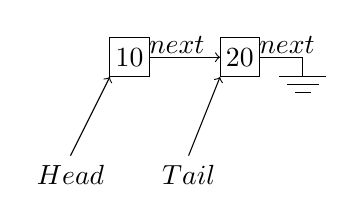
\begin{tikzpicture}
      \draw (0, 0) rectangle(.5, .5);
      \draw (.25, .25) node{$10$};
      \draw[->] (.5, .25) -- (1.4, .25);
      \draw (2.25, .4) node{$next$};
      \draw (-.5, -1) node[anchor=north]{$Head$};
      \draw (1, -1) node[anchor=north]{$Tail$};
      \draw[->] (-.5, -1) -- (0, 0);
      \draw[->] (1, -1) -- (1.4, 0);
      
      \draw (1.4, 0) -- (1.9, 0) -- (1.9, .5) -- (1.4, .5) --cycle;
      \draw (1.65, .25) node{$20$};
      \draw (.85, .4) node{$next$};
      \draw (1.9, .25) -- (2.45, .25) -- (2.45, 0);
      \draw (2.15, 0) -- (2.75, -0);
      \draw (2.25, -.1) -- (2.65, -.1);
      \draw (2.35, -.2) -- (2.55, -.2);
    \end{tikzpicture}
  \end{center}
\end{frame}
\begin{frame}[fragile]{When head is not euqal to tail}
  We copy data of \texttt{head}. Copy head to a temporary pointer
  \texttt{temp}. Then set \texttt{head} to point to next node and free
  from the temporary pointer \texttt{temp}. The we free \texttt{temp}.
  The order is important.
  \begin{center}
    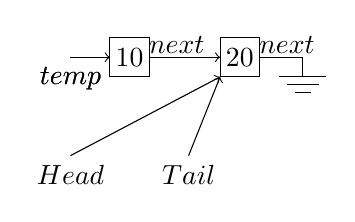
\begin{tikzpicture}
      \draw (0, 0) rectangle(.5, .5);
      \draw (.25, .25) node{$10$};
      \draw[->] (.5, .25) -- (1.4, .25);
      \draw (2.25, .4) node{$next$};
      \draw (-.5, -1) node[anchor=north]{$Head$};
      \draw (1, -1) node[anchor=north]{$Tail$};
      \draw[->] (-.5, -1) -- (1.4, 0);
      \draw[->] (1, -1) -- (1.4, 0);
      \draw (-.5, .25) node[anchor=north]{$temp$};
      \draw[->] (-.5, .25) -- (0, .25);
      
      \draw (-.5, .25) node[anchor=north]{$temp$};
      \draw (1.4, 0) -- (1.9, 0) -- (1.9, .5) -- (1.4, .5) --cycle;
      \draw (1.65, .25) node{$20$};
      \draw (.85, .4) node{$next$};
      \draw (1.9, .25) -- (2.45, .25) -- (2.45, 0);
      \draw (2.15, 0) -- (2.75, -0);
      \draw (2.25, -.1) -- (2.65, -.1);
      \draw (2.35, -.2) -- (2.55, -.2);
    \end{tikzpicture}
  \end{center}
\end{frame}
\begin{frame}[fragile]{When head is euqal to tail}
  We copy data of \texttt{head}. Copy head to a temporary pointer
  \texttt{temp}. Then set \texttt{head} and \texttt{tail} to \texttt{NULL}
  The we free \texttt{temp}.
  The order is important.
  \begin{center}
    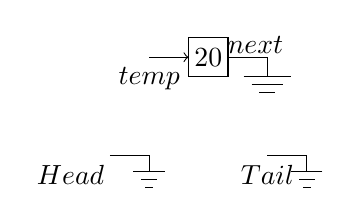
\begin{tikzpicture}
      \draw (0,0) rectangle(.5, .5);
      \draw (.25, .25) node{$20$};
      \draw (-1, -1) -- (-.5, -1) -- (-.5, -1.2);
      \draw (1, -1) -- (1.5, -1) -- (1.5, -1.2);
      \draw (.5, .25) -- (1, .25) -- (1, 0);
      \draw (.85, .4) node{$next$};
      \draw (.7, 0) -- (1.3, 0);
      \draw (.8, -.1) -- (1.2, -.1);
      \draw (.9, -.2) -- (1.1, -.2);
      \draw (-1.5, -1) node[anchor=north]{$Head$};
      \draw (1, -1) node[anchor=north]{$Tail$};
      \draw (-.7, -1.2) -- (-.3, -1.2);
      \draw (-.6, -1.3) -- (-.4, -1.3);
      \draw (-.55, -1.4) -- (-.45, -1.4);
      \draw (1.7, -1.2) -- (1.3, -1.2);
      \draw (1.6, -1.3) -- (1.4, -1.3);
      \draw (1.55, -1.4) -- (1.45, -1.4);
      \draw (-.5, .25) node[anchor=north]{$temp$};
      \draw[->] (-.5, .25) -- (0, .25);
    \end{tikzpicture}
  \end{center}
\end{frame}

\end{document}
